\documentclass[man,floatsintext]{apa6}
\usepackage{lmodern}
\usepackage{amssymb,amsmath}
\usepackage{ifxetex,ifluatex}
\usepackage{fixltx2e} % provides \textsubscript
\ifnum 0\ifxetex 1\fi\ifluatex 1\fi=0 % if pdftex
  \usepackage[T1]{fontenc}
  \usepackage[utf8]{inputenc}
\else % if luatex or xelatex
  \ifxetex
    \usepackage{mathspec}
  \else
    \usepackage{fontspec}
  \fi
  \defaultfontfeatures{Ligatures=TeX,Scale=MatchLowercase}
\fi
% use upquote if available, for straight quotes in verbatim environments
\IfFileExists{upquote.sty}{\usepackage{upquote}}{}
% use microtype if available
\IfFileExists{microtype.sty}{%
\usepackage{microtype}
\UseMicrotypeSet[protrusion]{basicmath} % disable protrusion for tt fonts
}{}
\usepackage{hyperref}
\hypersetup{unicode=true,
            pdftitle={Language use shapes cultural norms: Large scale evidence from gender},
            pdfauthor={Molly Lewis~\& Gary Lupyan},
            pdfkeywords={cultural norms, implicit association task (IAT), gender},
            pdfborder={0 0 0},
            breaklinks=true}
\urlstyle{same}  % don't use monospace font for urls
\usepackage{graphicx,grffile}
\makeatletter
\def\maxwidth{\ifdim\Gin@nat@width>\linewidth\linewidth\else\Gin@nat@width\fi}
\def\maxheight{\ifdim\Gin@nat@height>\textheight\textheight\else\Gin@nat@height\fi}
\makeatother
% Scale images if necessary, so that they will not overflow the page
% margins by default, and it is still possible to overwrite the defaults
% using explicit options in \includegraphics[width, height, ...]{}
\setkeys{Gin}{width=\maxwidth,height=\maxheight,keepaspectratio}
\IfFileExists{parskip.sty}{%
\usepackage{parskip}
}{% else
\setlength{\parindent}{0pt}
\setlength{\parskip}{6pt plus 2pt minus 1pt}
}
\setlength{\emergencystretch}{3em}  % prevent overfull lines
\providecommand{\tightlist}{%
  \setlength{\itemsep}{0pt}\setlength{\parskip}{0pt}}
\setcounter{secnumdepth}{0}
% Redefines (sub)paragraphs to behave more like sections
\ifx\paragraph\undefined\else
\let\oldparagraph\paragraph
\renewcommand{\paragraph}[1]{\oldparagraph{#1}\mbox{}}
\fi
\ifx\subparagraph\undefined\else
\let\oldsubparagraph\subparagraph
\renewcommand{\subparagraph}[1]{\oldsubparagraph{#1}\mbox{}}
\fi

%%% Use protect on footnotes to avoid problems with footnotes in titles
\let\rmarkdownfootnote\footnote%
\def\footnote{\protect\rmarkdownfootnote}


  \title{Language use shapes cultural norms: Large scale evidence from gender}
    \author{Molly Lewis\textsuperscript{1,2}~\& Gary Lupyan\textsuperscript{1}}
    \date{}
  
\shorttitle{Language use shapes cultural norms}
\affiliation{
\vspace{0.5cm}
\textsuperscript{1} University of Wisconsin-Madison\\\textsuperscript{2} University of Chicago}
\keywords{cultural norms, implicit association task (IAT), gender\newline\indent Word count: X}
\usepackage{csquotes}
\usepackage{upgreek}
\captionsetup{font=singlespacing,justification=justified}

\usepackage{longtable}
\usepackage{lscape}
\usepackage{multirow}
\usepackage{tabularx}
\usepackage[flushleft]{threeparttable}
\usepackage{threeparttablex}

\newenvironment{lltable}{\begin{landscape}\begin{center}\begin{ThreePartTable}}{\end{ThreePartTable}\end{center}\end{landscape}}

\makeatletter
\newcommand\LastLTentrywidth{1em}
\newlength\longtablewidth
\setlength{\longtablewidth}{1in}
\newcommand{\getlongtablewidth}{\begingroup \ifcsname LT@\roman{LT@tables}\endcsname \global\longtablewidth=0pt \renewcommand{\LT@entry}[2]{\global\advance\longtablewidth by ##2\relax\gdef\LastLTentrywidth{##2}}\@nameuse{LT@\roman{LT@tables}} \fi \endgroup}



\authornote{Portions of this manuscript appeared in Lewis \&
Lupyan, 2018, Cog. Sci Proceedings.

Correspondence concerning this article should be addressed to Molly
Lewis, . E-mail:
\href{mailto:mollyllewis@gmail.com}{\nolinkurl{mollyllewis@gmail.com}}}

\abstract{

}

\usepackage{amsthm}
\newtheorem{theorem}{Theorem}[section]
\newtheorem{lemma}{Lemma}[section]
\theoremstyle{definition}
\newtheorem{definition}{Definition}[section]
\newtheorem{corollary}{Corollary}[section]
\newtheorem{proposition}{Proposition}[section]
\theoremstyle{definition}
\newtheorem{example}{Example}[section]
\theoremstyle{definition}
\newtheorem{exercise}{Exercise}[section]
\theoremstyle{remark}
\newtheorem*{remark}{Remark}
\newtheorem*{solution}{Solution}
\begin{document}
\maketitle

\section{Introduction}\label{introduction}

The language we use to communicate a message shapes how our listener
interprets that message (Fausey \& Boroditsky, 2010; Loftus \& Palmer,
1974; Tversky \& Kahneman, 1981). A listener, for example, is more
likely to infer that a person is at fault if the event is described
actively (e.g., \enquote{she ignited the napkin}), as opposed to
passively (e.g., \enquote{the napkin ignited}). The formative power of
language is perhaps most potent in shaping meanings that necessarily
must be learned from others: cultural norms. In the present paper, we
consider one type of cultural norm---gender---and examine the extent to
which differences in language use may lead to cross-cultural differences
in understandings of gender.

Gender provides a useful case study of the relationship between language
and thought for several reasons. First, more abstract domains like
gender may be more subject to the influence of language relative to more
perceptually grounded domains like natural kinds (Boroditsky, 2001).
Second, many languages encode the gender of speakers and addressees
explicitly in their grammar. Third, a large body of evidence suggests
that language plays a key role in transmitting social knowledge to
children (e.g., Master, Markman, \& Dweck, 2012). And, fourth, gender
norms are highly variable across cultures and have clear and important
social implications.

For our purposes, we define the hypothesis space of possible
relationships between language and gender norms with two broad extremes:
(1) language reflects a pre-existing gender bias in its speakers
(\emph{language-as-reflection hypothesis}); (2) language causally
influences gender biases (\emph{language-as-causal hypothesis}). We
assume that the language-as-reflection hypothesis is true to some
extent: some of the ways we talk about gender reflect our knowledge and
biases acquired independently of language. For example, we may observe
that most nurses are women, and therefore be more likely to use a female
pronoun to refer to a nurse of an unknown gender. Our goal here is to
understand the extent to which language may also exert a causal
influence on conceptualizations of gender.

In particular, we explore two possible mechanisms by which the way we
speak may influence notions of gender. The first is through the overt
grammatical marking of gender, particularly on nouns, which is
obligatory in roughly one quarter of languages (e.g., in Spanish,
``nina'' (girl) and ``enfermera'' (nurse) both take the gender marker
\emph{-a} to indicate grammatical femininity; Corbett, 1991). Because
grammatical gender has a natural link to the real world, speakers may
assume that grammatical markers are meaningful even when applied to
inanimate objects that do not have a biological sex. In addition, the
mere presence of obligatory marking of grammatical gender may promote
bias by making the dimension of gender more salient to speakers.

A second route by which language may shape gender norms is via word
co-occurrences. Words that tend to occur in similar contexts in language
may lead speakers to assume---either implicitly or explicitly---that
they have similar meanings. For example, statistically, the word
\enquote{nurse} occurs in many of the same contexts as the pronoun
\enquote{her,} providing an implicit link between these two concepts
that may lead to a bias to assume that nurses are female. This second
route may be particularly influential because the bias is encoded in
language in a way that is more implicit than grammatical markers of
gender and thus more difficult to reject.

An existing body of experimental work points to a link between language
and psychological gender bias in both adults (e.g., Phillips \&
Boroditsky, 2003) and children (e.g., Sera, Berge, \& Castillo Pintado,
1994). For example, Phillips and Boroditsky (2003) asked Spanish-English
and German-English adult bilinguals to make similarity judgements
between pairs of pictures depicting an object with a natural gender
(e.g., a bride) and one without (e.g., a toaster). They found that
participants rated pairs as more similar when the pictures matched in
grammatical gender in their native language. While these types of
studies provide suggestive evidence for a causal link between language
and psychological gender bias, they are limited by the fact that they
typically only compare speakers of 2-3 different languages and measure
bias in a way that is subject to demand characteristics.

In what follows, we ask whether the way gender is encoded linguistically
across 25 different languages predicts cross-cultural variability in a
particular manifestation of a gender bias---the bias to associate men
with careers and women with family. We begin by describing our
cross-cultural dataset in psychological gender bias. In Study 1, we use
semantic-embedding models to examine whether variability in lexical
semantics predicts variability in psychological gender biases. In Study
2, we ask whether the presence of grammatical gender in a language is
associated with greater implicit gender bias. Together, our data suggest
that both language statistics and language structure likely play a
causal role in shaping culturally-specific notions of gender.

\section{Description of Cross-Cultural IAT
Dataset}\label{description-of-cross-cultural-iat-dataset}

To quantify cross-cultural gender bias, we used data from a large-scale
administration of an Implicit Association Task (IAT; Greenwald, McGhee,
\& Schwartz, 1998) by Project Implicit
(\url{https://implicit.harvard.edu/implicit/}; Nosek, Banaji, \&
Greenwald, 2002). The IAT measures the strength of respondents' implicit
associations between two pairs of concepts (e.g.,
male-career/female-family vs.~male-family/female-career) accessed via
words (e.g., \enquote{man,} \enquote{business}). The underlying
assumption of the IAT is that words denoting more similar meanings
should be easier to pair together compared to more dissimilar pairs.

Meanings are paired in the task by assigning them to the same response
keys in a two-alternatie forced-choice categorization task. In the
critical blocks of the task, meanings are assigned to keys in a way that
is either bias-congruent (i.e.~Key A = male/career; Key B =
female/family) or bias-incongruent (i.e.~Key A = male/family; Key B =
female/career). Participants are then presented with a word related to
one of the four concepts and asked to classify it as quickly as
possible. Slower reaction times in the bias-incongruent blocks relative
to the bias-congruent blocks are interpreted as indicating an implicit
association between the corresponding concepts (i.e.~a bias to associate
male with career and female with family).

In the present study, we analyzed a dataset of gender-career IAT scores
collected by Project Implicit between 2005 and 2016. We restricted our
sample based on participants' reaction times and error rates using the
same criteria described in Nosek, Banjai, and Greenwald (2002, pg.~104).
We only analyzed data for countries that had at least 400 participants.
Our final sample included 769,353 participants from 40 countries, with a
median of 1,302 participants per country. Note that although the
respondents were from largely non-English speaking countries, the IAT
was conducted in English. We do not have language background data from
the participants, but we assume that most respondents from non-English
speaking countries were native speakers of the dominant language of the
country and L2 speakers of English.

Several measures have been used in the literature to quantify the
strength of the bias from participants' responses on congruent and
incongruent blocks on the IAT. Here, we used the most robust measure,
D-score, which measures the difference between critical blocks for each
participant while controlling for individual differences in response
time (Greenwald, Nosek, \& Banaji, 2003). In addition to the implicit
measure, we also analyzed an explicit measure of gender bias. After
completing the IAT, participants were asked, \enquote{How strongly do
you associate the following with males and females?} for both the words
\enquote{career} and \enquote{family.} Participants indicated their
response on a Likert scale ranging from \emph{female} (1) to \emph{male}
(7). We calculated an explicit gender bias score for each participant as
the Career response minus the Family response, such that greater values
indicate a greater bias to associate males with career.

\begin{figure}[t]

{\centering 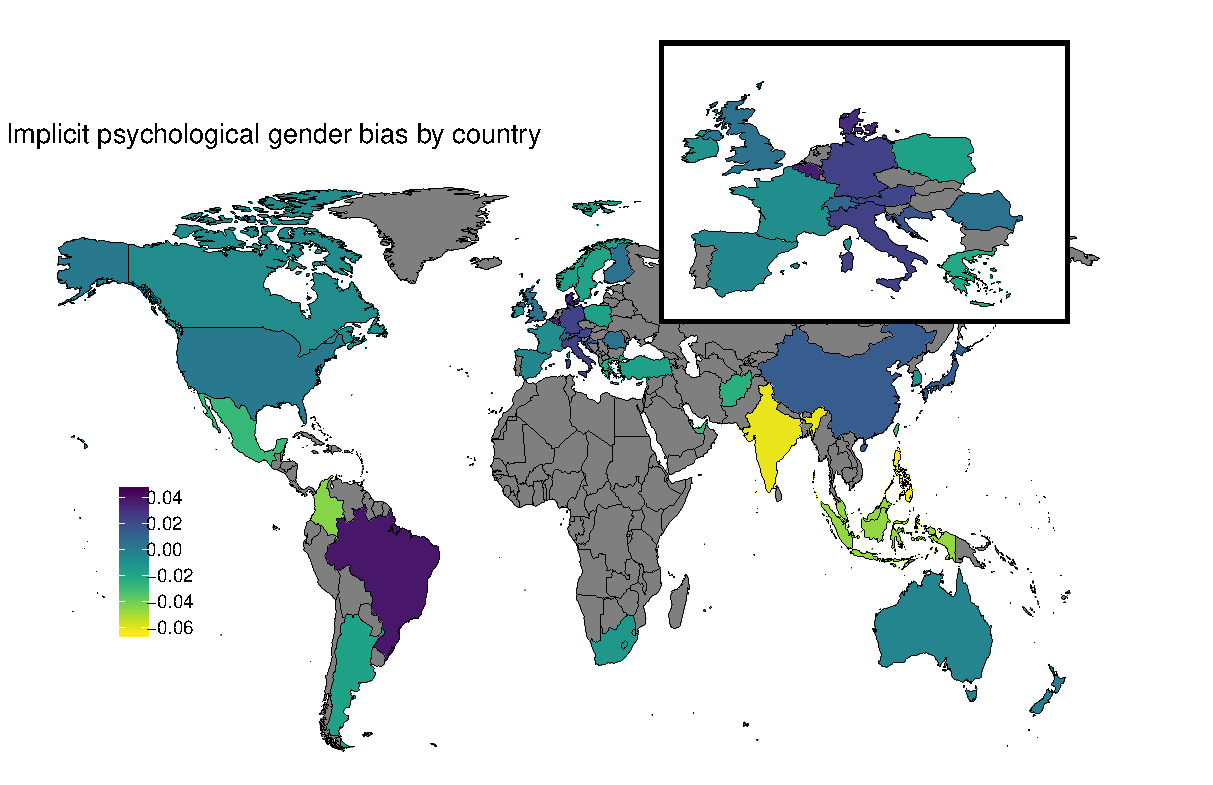
\includegraphics{/Users/mollylewis/Documents/research/Projects/1_in_progress/IATLANG/writeup/journal/figs/map_figure} 

}

\caption{Residualized gender bias by country as measured by the IAT. Larger values indicate a larger bias to associate women with the concept of family and men with the concept of career. Countries in grey correspond to countries for which there was insufficient data to estimate the country-level gender bias.}\label{fig:mapplot}
\end{figure}

At the participant level, implicit bias scores were correlated with
participant age such that older participants tended to have a large
gender bias compared to younger participants (\emph{r} = 0.06, \emph{p}
\textless{} .0001). We also found that implicit bias scores varied as a
function of participant sex, such that males (\emph{M} = 0.32, \emph{SD}
= 0.39) showing a smaller implicit gender bias than females (\emph{M} =
0.42, \emph{SD} = 0.36; \emph{t} = 105.97, \emph{p} \textless{} .0001),
a pattern consistent with previous findings (Nosek et al., 2002).
Finally, implicit bias scores varied as a function of block order on the
IAT task (\emph{t} = -114.59, \emph{p} \textless{} .0001). For the
present purposes, our goal was to estimate gender bias at the country
level. To account for covariates of gender bias, we calculated a
residual implicit bias score for each participant, controlling for
participant age, participant sex, and block order. We also calculated a
residual explicit bias score controling for the same set of variables.
We then averaged across participants to estimate the country-level
gender bias. Figure 1 shows residualized implicit gender bias by country
(\emph{M} = -0.01; \emph{SD} = 0.03). Implicit gender biases were
moderately correlated with explicit gender biases at the level of
participants (\emph{r} = 0.16, \emph{p} \textless{} .0001) but not
countries (\emph{r} = 0.27, \emph{p} = 0.09).

We compared our residual country-level implicit and explicit gender
biases to an objective measure of gender equality that is measured for
each country by the United Nations Educational, Scientific and Cultural
Organization (UNESCO): the percentage of women among science,
technology, engineering, and mathematics (STEM) graduates in tertiary
education (Miller, Eagly, \& Linn, 2015; Stoet \& Geary, 2018).
Consistent with previous research (Miller et al., 2015), we found that
implicit gender bias was negatively correlated with percentage of women
in STEM fields: Countries with a smaller gender bias tended to have more
women in STEM fields (\emph{r} = -0.47, \emph{p} = 0.01). There was not
a relationship between explicit gender bias and percentage of women in
STEM fields (\emph{r} = 0.16, \emph{p} = 0.43). In addition, we found a
strong correlation between the median age of a country, as measured by
the CIA factbook (2017), and residual implicit bias: Countries with
older populations tended to have larger gender biases (\emph{r} = 0.60,
\emph{p} \textless{} .0001).

In sum, we replicate previously-reported patterns of gender bias in the
gender-career IAT literature, with roughly comparable effect sizes
(c.f.~Nosek, et al., 2002). The weak correlation between explicit and
implicit measures is consistent with claims that these two measures tap
into different cognitive constructs (Forscher et al., 2016). In
addition, we find that an objective measure of gender equality---female
enrollment in STEM fields---is predictive of psychological gender bias.

\section{Study 1: Gender bias and
semantics}\label{study-1-gender-bias-and-semantics}

In Study 1, we ask whether participants' implicit and explicit gender
biases are correlated with the biases in the semantic structure of their
native languages. For example, are the semantics of the words
\enquote{woman} and \enquote{family} more similar in Spanish than in
English? Both the language-as-reflection and language-as-causal
hypotheses predict a positive correlation between psychological and
semantic gender biases.

As a model of word meanings, we use large-scale distributional semantics
models derived from auto-encoding neural networks trained on large
corpora of text. The underlying assumption of these models is that the
meaning of a word can be described by the words it tends to co-occur
with---an approach known as distributional semantics (Firth, 1957).
Under this approach, a word like \enquote{dog} is represented as more
similar to \enquote{hound} than to \enquote{banana} because
\enquote{dog} co-occurs with words more in common with \enquote{hound}
than \enquote{banana.}

Recent developments in machine learning allow the idea of distributional
semantics to be implemented in a way that takes into account many
features of local language structure while remaining computationally
tractable. The best known of these word embedding models is
\emph{word2vec} (Mikolov, Chen, Corrado, \& Dean, 2013). The model takes
as input a corpus of text and outputs a vector for each word
corresponding to its semantics. From these vectors, we can derive a
measure of the semantic similarity between two words by taking the
distance between their vectors (e.g., cosine distance).

As it turns out, the biases previously reported using IAT tests can be
predicted from distributional semantics models like word2vec using
materials identical to those used in the IAT experiments. Caliskan,
Bryson, and Narayanan (2017; henceforth \emph{CBN}) measured the
distance in vector space between the words presented to participants in
the IAT task. CBN found that these distance measures were highly
correlated with reaction times in the behavioral IAT task. For example,
CBN find a bias to associate males with career and females with family
in the career-gender IAT, suggesting that the biases measured by the IAT
are also found in the lexical semantics of natural language.

CBN only measured semantic biases in English, however. In Study 1, we
use the method described by CBN to measure gender bias in the range of
first languages spoken by participants in the Project Implicit dataset
by using models trained on those languages. In Study 1a, we first
validate word embedding measures of gender bias by comparing them to
explicit human judgements of gender bias. In Study1b, we apply this
method to models trained on text in other languages. We find that the
implicit gender biases reported in Study 1 for individual countries are
correlated with the biases found in the semantics of the natural
language spoken by those participants.

\subsection{Study 1a: Word embeddings as a measure of psychological
gender
bias}\label{study-1a-word-embeddings-as-a-measure-of-psychological-gender-bias}

To validate word embeddings as a measure of psychological gender bias,
we asked whether words that were closely associated with males in the
word embedding models tended to be rated by human participants as being
more male biased. We found human and word-embedding estimates of gender
bias to be highly correlated.

\subsubsection{Methods}\label{methods}

We used an existing set of word norms in which participants were asked
to rate \enquote{the gender associated with each word} on a Likert scale
ranging from \emph{very feminine} (1) to \emph{very masculine} (7;
Scott, Keitel, Becirspahic, Yao, \& Sereno, 2018). We compared these
gender norms to estimates of gender bias from a word embedding model
pre-trained on the corpus of English Wikipedia using the fastText
algorithm (a variant of word2vec; Bojanowski, Grave, Joulin, \& Mikolov,
2016; Joulin, Grave, Bojanowski, \& Mikolov, 2016). The model contains
2,519,370 words with each word represented by a 300 dimensional vector.
To calculate a gender scores from the word embeddings, for each word we
calculated the average cosine distance to a set of male words
(\enquote{male}, \enquote{man}, \enquote{he}, \enquote{boy},
\enquote{his}, \enquote{him}, \enquote{son}, \enquote{brother}) and the
average cosine similarity to a set of female words (\enquote{female},
\enquote{woman}, \enquote{she}, \enquote{girl}, \enquote{hers},
\enquote{her}, \enquote{daughter}, \enquote{sister}). A gender score for
each word was then obtained by taking the difference of the similarity
estimates (mean male similarity - mean female similarity), such that
larger values indicated a stronger association with males. There were
4671 words in total that overlapped between the two data sources.

\subsubsection{Results and Discussion}\label{results-and-discussion}

Estimates of gender bias from word embeddings (\emph{M} = 0; \emph{SD} =
0.03) and human judgements (\emph{M} = 4.10; \emph{SD} = 0.92) were
highly correlated (\emph{r} = 0.59; \emph{p} \textless{} .0001; Fig. 2).

\begin{figure}
\centering
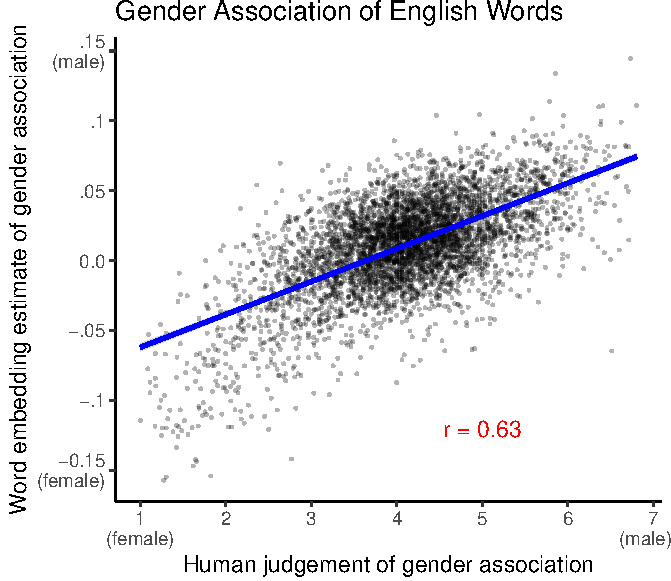
\includegraphics{iat_lang_files/figure-latex/unnamed-chunk-11-1.pdf}
\caption{\label{fig:unnamed-chunk-11}Word embedding estimates of gender bias
as a function of human judgements of gender bias (Study 1a). Each point
corresponds to a word. Larger numbers indicate stronger association with
males. Blue line shows linear fit and the error band corresponds to a
standard error (too small to be visible).}
\end{figure}

\subsection{Study 1b: Cross-linguistic gender bias
semantics}\label{study-1b-cross-linguistic-gender-bias-semantics}

With our corpus validated, we next turn toward examining the
relationship between psychological and linguistic gender biases. In
Study 1b, we estimate the magnitude of the gender-career bias in each of
the languages spoken in the countries described in the Project Implicit
dataset and compare it with estimates of behavioral gender bias from the
Project Implicit data set. If language plays a causal role in shaping
psychological gender biases, we predict that participants who speak a
language with larger gender bias will tend to have a larger
psychological gender bias.

\subsubsection{Methods}\label{methods-1}

For each country represented in our analysis of the Project Implicit, we
identified the most frequently spoken language in each country using the
CIA factbook (2017). This included a total of 27 unique languages. For
two languages, Zulu and Tagalog, the corpora that the models were
trained on (see below) was insufficiently large to be reliable, and so
we excluded these languages from our analysis. Our final sample included
25 languages, representing XX different language families..

We obtained translations from native speakers into each these languages
for a set of 8 female and 8 male target words (identical to Study 1a), a
set of 8 attribute words associated with the concept \enquote{career}
(\enquote{career,} \enquote{executive,} \enquote{management,}
\enquote{professional,} \enquote{corporation,} \enquote{salary,}
\enquote{office,} \enquote{business}) and 8 attribute words associated
with the concept \enquote{family} (\enquote{family,} \enquote{home,}
\enquote{parents,} \enquote{children,} \enquote{cousins,}
\enquote{marriage,} \enquote{wedding,} \enquote{relatives}). Our word
lists are identical to the stimuli in the Project Implicit gender-career
IAT behavioral task (Nosek et al., 2002) with one slight modification.
In the behavioral task, proper names were used to cue the male and
female categories (e.g.~\enquote{John,} \enquote{Amy}), but because
there are not direct translation equivalents of proper names, we instead
used a set of generic gendered words which had been previously used for
a different version of the gender IAT (e.g., ``man,'' ``woman;'' Nosek
et al., 2002).

We used these translations to calculate a gender bias effect size from
word embedding models trained on text in each language. Our effect size
measure is a standardized difference score of the relative similarity of
the target words to the target attributes (i.e.~relative similarity of
male to career vs.~relative similarity of female to career). Our effect
size measure is identical to that used by CBN with one exception (see SM
for replication of CBN on our corpora). Namely, for languages with
grammatically gendered attribute words (e.g., ninas for female children
in Spanish), we calculated the relationship between target words and
attribute words of the same gender (i.e. \enquote{man} to
\enquote{ninos} and \enquote{woman} to \enquote{ninas}). In cases where
there were multiple translations for a word, or the translation
contained multiple words, we averaged across words such that each of our
target words was associated with a single vector in each language. Our
effect size measure is analogous to the to the behavioral effect size
measure obtained from the IAT task in Project Implicit, where larger
values indicate larger gender bias.

We calculated gender bias estimates based on models trained on two
different corpora: Wikipedia (Bojanowski et al., 2016) and Subtitles
{[}where are these from?{]}. These two models capture different types of
XX. We then compared the effect size of the linguistic gender bias to
the behavioral IAT gender bias estimated from Project Implicit,
averaging across countries that speak whose participants speak the same
language.

\subsubsection{Results}\label{results}

\begin{figure}
\centering
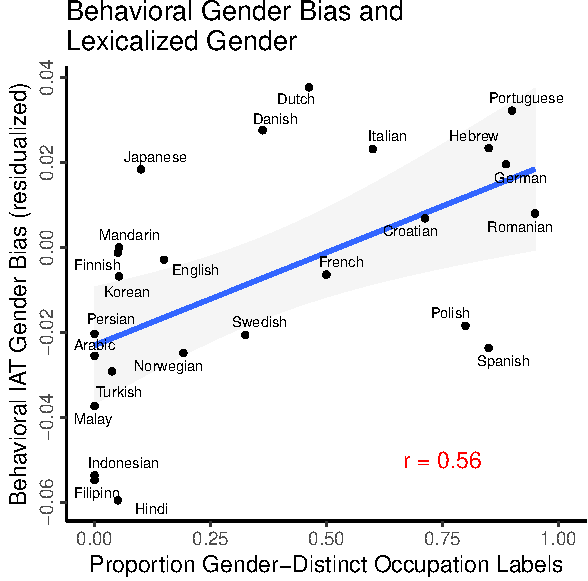
\includegraphics{iat_lang_files/figure-latex/unnamed-chunk-14-1.pdf}
\caption{\label{fig:unnamed-chunk-14}Residualized behavioral IAT gender bias
as a function of semantic IAT gender bias by language (Study 1b).
Semantic biases are estimated from models trained on each language using
a subtitle corpus (left) and a sample of Wikipedia (right). Larger
values indicate a larger bias to associate men with the concept of
career and women with the concept of family. Error bands correspond to
standard errors.}
\end{figure}

At the level of languages, our estimate of gender bias in the semantics
of each language was positively correlated the implicit gender bias of
participants who spoke that language (\emph{r} = 0.36; \emph{p} = 0.08;
Fig. 3). Importantly, this relationship held when controling for median
country age in a linear model (\(\beta\)= 0.02; \emph{SE} = 0.01,
\emph{p} = 0.09). Semantic IAT gender bias was not correlated with
explicit gender bias (\emph{r} = 0.29; \emph{p} = 0.16). {[}Percentage
women in stem and language are marginal p = .06{]}. Table 1 shows the
language-level correlations between all variables.

\begin{table}

\caption{\label{tab:corrtable}Correlation (Pearson's r) for all measures in Study 1 at the level of languages. Asterisks indicate significance at the .05 level.}
\centering
\fontsize{10}{12}\selectfont
\begin{tabular}[t]{l>{\raggedleft\arraybackslash}p{2.5cm}>{\raggedleft\arraybackslash}p{2.5cm}>{\raggedleft\arraybackslash}p{2.5cm}>{\raggedleft\arraybackslash}p{2.5cm}lrrrrlrrrrlrrrrlrrrr}
\toprule
 & Language IAT
(Subtitles) & Language IAT 
 (Wikipedia) & Residualized 
Explicit Bias & Residualized 
Behavioral IAT\\
\midrule
Language IAT (Subtitles) &  &  &  & \\
Language IAT (Wikipedia) & .58** &  &  & \\
Residualized Explicit Bias & .04 & .29 &  & \\
Residualized Behavioral IAT & .42 & .36 & .14 & \\
Perecent Women in Stem & -.40 & -.19 & .30 & -.44\\
\bottomrule
\end{tabular}
\end{table}

\subsubsection{Discussion}\label{discussion}

\section{Study 2: Gender bias and
grammar}\label{study-2-gender-bias-and-grammar}

The findings in Study 1 are consistent with both the language-as-causal
and language-as-reflection hypotheses. In Study 2, we try to distinguish
between the two hypotheses by asking whether there is a relationship
between psychological gender bias and language along a linguistic
dimension that is unlikely to be a subject of rapid change---namely,
grammatical gender. While of course grammars do change over time, they
are less malleable than the meanings of individual words, and thus less
likely to be affected by psychological biases. We predict, therefore,
that if language causally influences psychological gender biases,
languages that encode gender grammatically will tend to have larger
psychological gender biases.

\subsubsection{Method}\label{method}

We coded each of the languages in our sample (Study 1) for grammatical
gender. We used a coarse binary coding scheme, categorizing a language
as encoding grammatical gender if it made any gender distinction on noun
classes (masculine, feminine, common or neuter), and as not encoding
gender grammatically otherwise.

\subsubsection{Results and Discussion}\label{results-and-discussion-1}

\begin{figure}
\centering
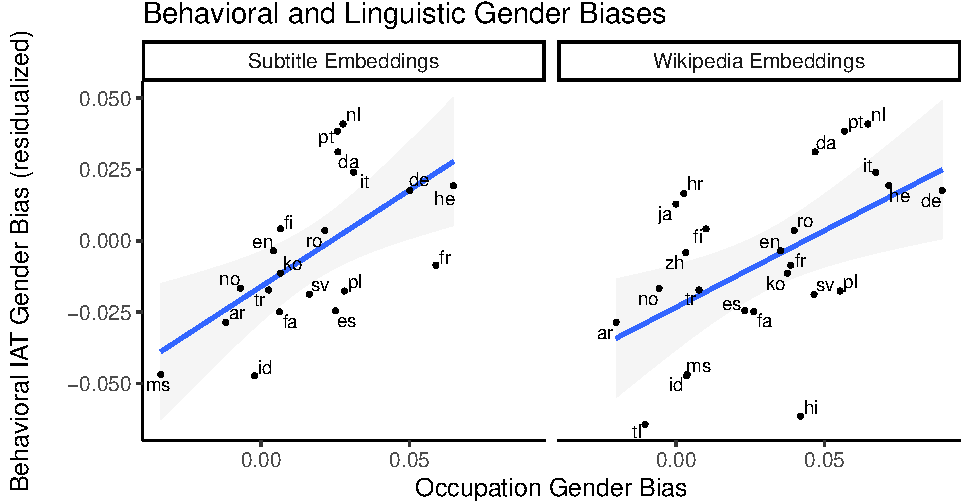
\includegraphics{iat_lang_files/figure-latex/unnamed-chunk-19-1.pdf}
\caption{\label{fig:unnamed-chunk-19}Residualized behavioral IAT gender bias
as a function of whether or not the language encodes grammatical gender.
Each label code corresponds to a language. The bold vertical line
corresponds to the group median, and the box width indicates the first
and third quartile.}
\end{figure}

\section{General Discussion}\label{general-discussion}

\newpage

\section{References}\label{references}

\begingroup
\setlength{\parindent}{-0.5in} \setlength{\leftskip}{0.5in}

\hypertarget{refs}{}
\hypertarget{ref-bojanowski2016enriching}{}
Bojanowski, P., Grave, E., Joulin, A., \& Mikolov, T. (2016). Enriching
word vectors with subword information.

\hypertarget{ref-boroditsky2001does}{}
Boroditsky, L. (2001). Does language shape thought?: Mandarin and
English speakers' conceptions of time. \emph{Cognitive Psychology},
\emph{43}(1), 1--22.

\hypertarget{ref-caliskan2017semantics}{}
Caliskan, A., Bryson, J. J., \& Narayanan, A. (2017). Semantics derived
automatically from language corpora contain human-like biases.
\emph{Science}, \emph{356}(6334), 183--186.

\hypertarget{ref-ciafactbook}{}
Central Intelligence Agency (CIA). (2017). The World Factbook. Retrieved
from
\url{https://www.cia.gov/library/publications/the-world-factbook/index.html}

\hypertarget{ref-corbett1991}{}
Corbett, G. G. (1991). \emph{Gender}. Cambridge: Cambridge University
Press.

\hypertarget{ref-epi}{}
\emph{EF English Proficiency Index}. (2017). Retrieved from
\url{https://www.ef.edu/epi/}

\hypertarget{ref-fausey2010subtle}{}
Fausey, C. M., \& Boroditsky, L. (2010). Subtle linguistic cues
influence perceived blame and financial liability. \emph{Psychonomic
Bulletin \& Review}, \emph{17}(5), 644--650.

\hypertarget{ref-firth1957synopsis}{}
Firth, J. (1957). A synopsis of linguistic theory 1930-1955 in studies
in linguistic analysis, philological society. Oxford.

\hypertarget{ref-forscher2016meta}{}
Forscher, P. S., Lai, C., Axt, J., Ebersole, C. R., Herman, M., Devine,
P. G., \& Nosek, B. A. (2016). A meta-analysis of change in implicit
bias.

\hypertarget{ref-greenwald1998measuring}{}
Greenwald, A. G., McGhee, D. E., \& Schwartz, J. L. (1998). Measuring
individual differences in implicit cognition: The implicit association
test. \emph{Journal of Personality and Social Psychology}, \emph{74}(6),
1464.

\hypertarget{ref-greenwald2003understanding}{}
Greenwald, A. G., Nosek, B. A., \& Banaji, M. R. (2003). Understanding
and using the Implicit Association Test: An improved scoring algorithm.
\emph{Journal of Personality and Social Psychology}, \emph{85}(2), 197.

\hypertarget{ref-joulin2016bag}{}
Joulin, A., Grave, E., Bojanowski, P., \& Mikolov, T. (2016). Bag of
tricks for efficient text classification. \emph{arXiv Preprint
arXiv:1607.01759}.

\hypertarget{ref-loftus1974reconstruction}{}
Loftus, E. F., \& Palmer, J. C. (1974). Reconstruction of automobile
destruction: An example of the interaction between language and memory.
\emph{Journal of Verbal Learning and Verbal Behavior}, \emph{13}(5),
585--589.

\hypertarget{ref-master2012thinking}{}
Master, A., Markman, E., \& Dweck, C. (2012). Thinking in categories or
along a continuum: Consequences for children's social judgments.
\emph{Child Development}, \emph{83}(4).

\hypertarget{ref-mikolov2013efficient}{}
Mikolov, T., Chen, K., Corrado, G., \& Dean, J. (2013). Efficient
estimation of word representations in vector space.

\hypertarget{ref-miller2015women}{}
Miller, D. I., Eagly, A. H., \& Linn, M. C. (2015). Women's
representation in science predicts national gender-science stereotypes:
Evidence from 66 nations. \emph{Journal of Educational Psychology},
\emph{107}(3), 631.

\hypertarget{ref-nosek2002harvesting}{}
Nosek, B. A., Banaji, M. R., \& Greenwald, A. G. (2002). Harvesting
implicit group attitudes and beliefs from a demonstration web site.
\emph{Group Dynamics: Theory, Research, and Practice}, \emph{6}(1), 101.

\hypertarget{ref-phillips2003can}{}
Phillips, W., \& Boroditsky, L. (2003). Can quirks of grammar affect the
way you think? Grammatical gender and object concepts. In
\emph{Proceedings of the 25th Annual Meeting of the Cognitive Science
Society} (pp. 928--933).

\hypertarget{ref-scott2018glasgow}{}
Scott, G. G., Keitel, A., Becirspahic, M., Yao, B., \& Sereno, S. C.
(2018). The glasgow norms: Ratings of 5,500 words on nine scales.
\emph{Behavior Research Methods}, 1--13.

\hypertarget{ref-sera1994grammatical}{}
Sera, M. D., Berge, C. A., \& Castillo Pintado, J. del. (1994).
Grammatical and conceptual forces in the attribution of gender by
English and Spanish speakers. \emph{Cognitive Development}, \emph{9}(3),
261--292.

\hypertarget{ref-stoet2018gender}{}
Stoet, G., \& Geary, D. C. (2018). The gender-equality paradox in
science, technology, engineering, and mathematics education.
\emph{Psychological Science}, \emph{29}(4), 581--593.

\hypertarget{ref-tversky1981framing}{}
Tversky, A., \& Kahneman, D. (1981). The framing of decisions and the
psychology of choice. \emph{Science}, \emph{211}(4481), 453--458.

\hypertarget{ref-whorf1945grammatical}{}
Whorf, B. (1945). Grammatical categories. \emph{Language}, 1--11.

\hypertarget{ref-wps}{}
Women, Peace and Security Index. (2017). Retrieved from
\url{https://giwps.georgetown.edu/}

\endgroup


\end{document}
